\section{}
Consider the transfer function
\begin{align*}
    G(s) = \frac{s}{10s - 1}
\end{align*}
Sketch the Bode plot of $G(s)$ by hand, using the Bode graph paper provided on eClass, then validate
your answer using MATLAB's bode command. Please include both plots with your answer.

\subsection*{Solution}
There are two factors, $s$ and $10s - 1$. For $10s-1$, $1/\tau = 0.1$.

By Matlab,
\begin{lstlisting}[language=Matlab]
G = tf([1 0], [10 -1]);
bode(G);
\end{lstlisting}
\begin{figure}[h]
    \centering
    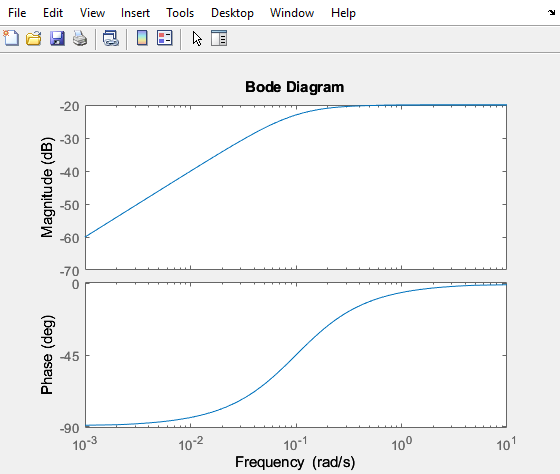
\includegraphics[width=0.8\linewidth]{Questions/Figures/Q1 Matlab Bode.png}
    \caption{Bode plot of $G(s)$ using Matlab}
    \label{fig:Q1 Matlab Bode}
\end{figure}

%put pdf in here
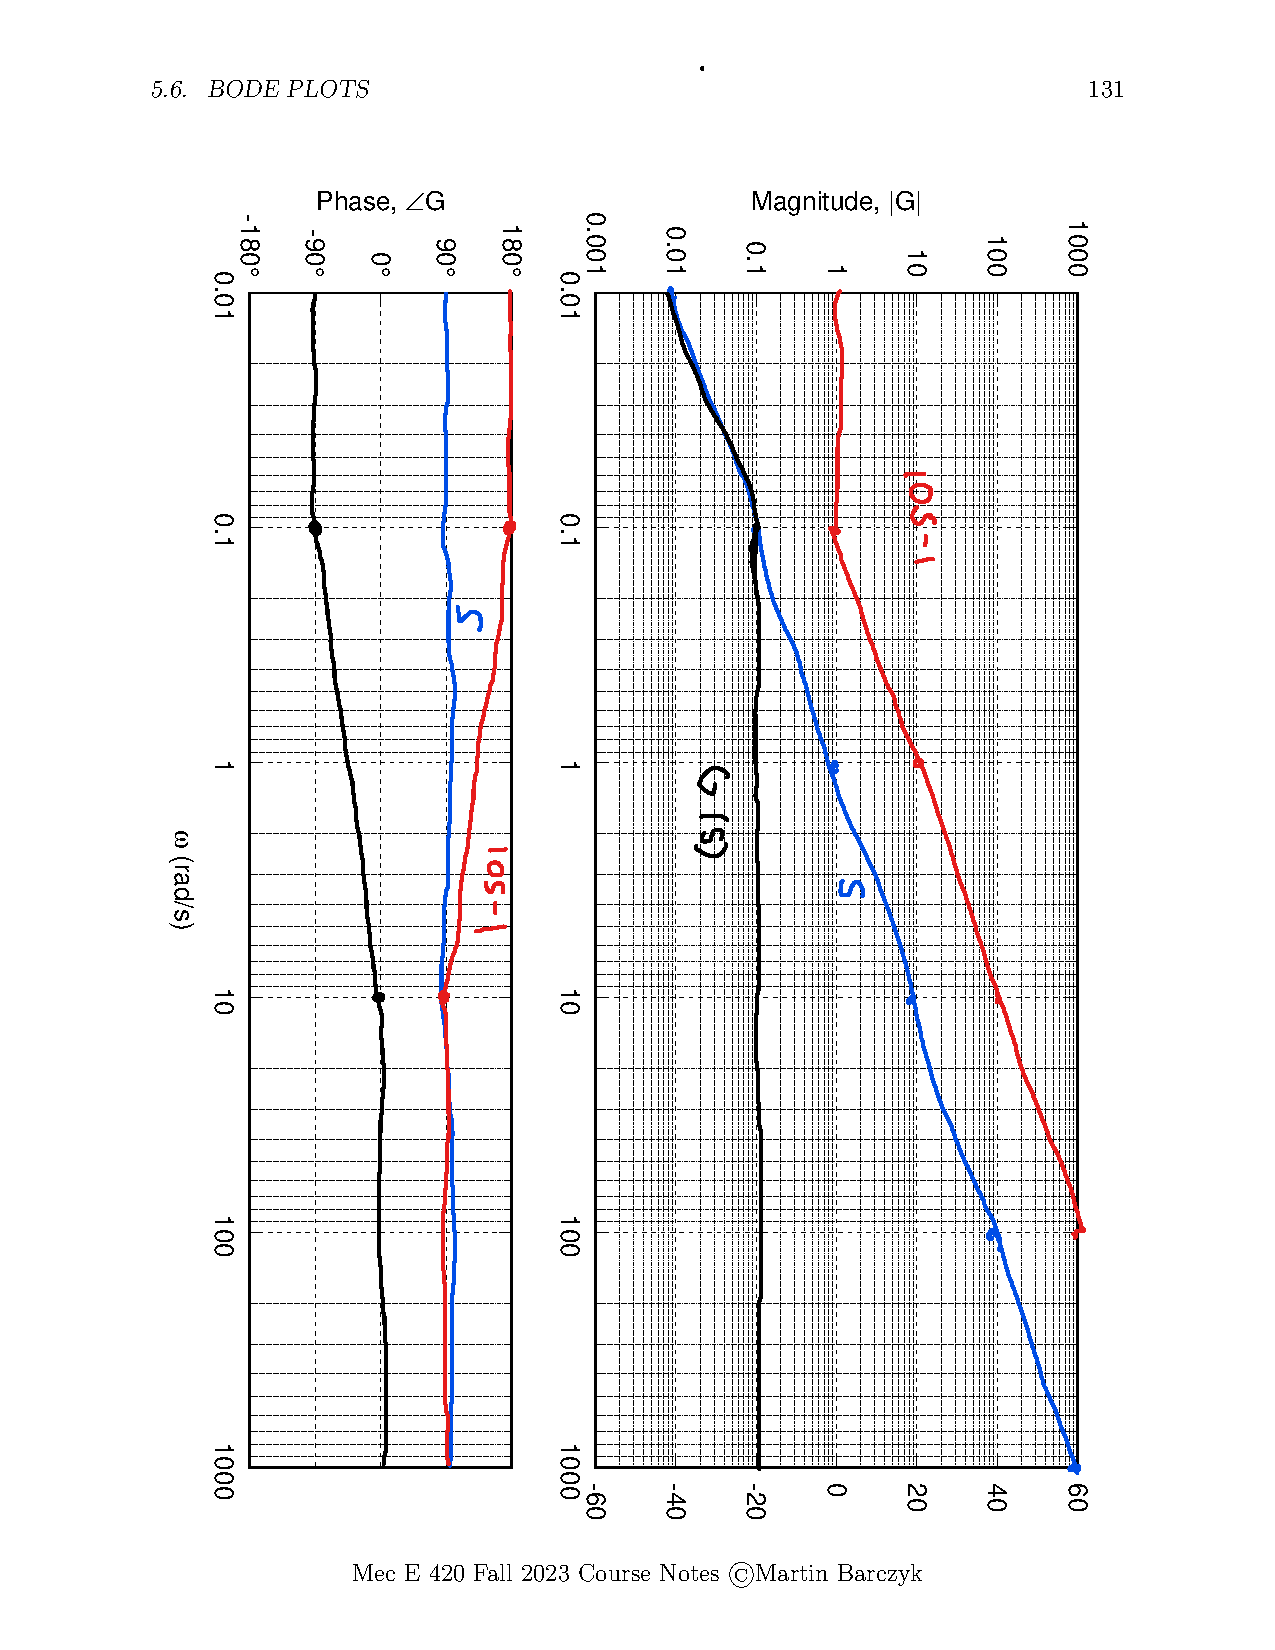
\includepdf[]{Q1 sketch.pdf}

